\section{Introduction}
\label{sec:introduction}

Today, Deep Learning jobs are a big part of workloads run by organizations, both
big and small. Often, DL training and inference tasks require GPUs and other
specialized hardware to run in reasonable times. Hence it is not uncommon to
have a cluster of GPU-enabled machines in production pipelines. Accordingly the
cloud infrastructure providers like AWS, GCP, Azure etc offer this choice to
their customers \cite{aws} \cite{GCP}. In addition, to manage costs, companies
also build and manage their own local cluster\cite{onprem}.


Inspite of the importance of DL jobs and large investments in the hardware
infrastructure, the software to manage them are mostly same as those used for
traditional big data jobs (like MapReduce). A typical workflow involves
packaging the job into a container like Docker and submitting it, along with
resource requirements, to a general purpose orchestration tool like Kubernetes
or YARN. Running DL jobs using this process leads to significant interactions
between the developer (a data scientist) and the underlying infrastructure as we
detail in Section []. On the other hand, GPUs remain under-utilised. For
instance, a startup that helps companies setup ML pipelines \cite{wab} notes
that the GPU utilization for over a third of their users is less than 15\%,
inspite of their users being experienced DL practitioners. There are two primary
causes:

\begin{figure}[htbp]
\centerline{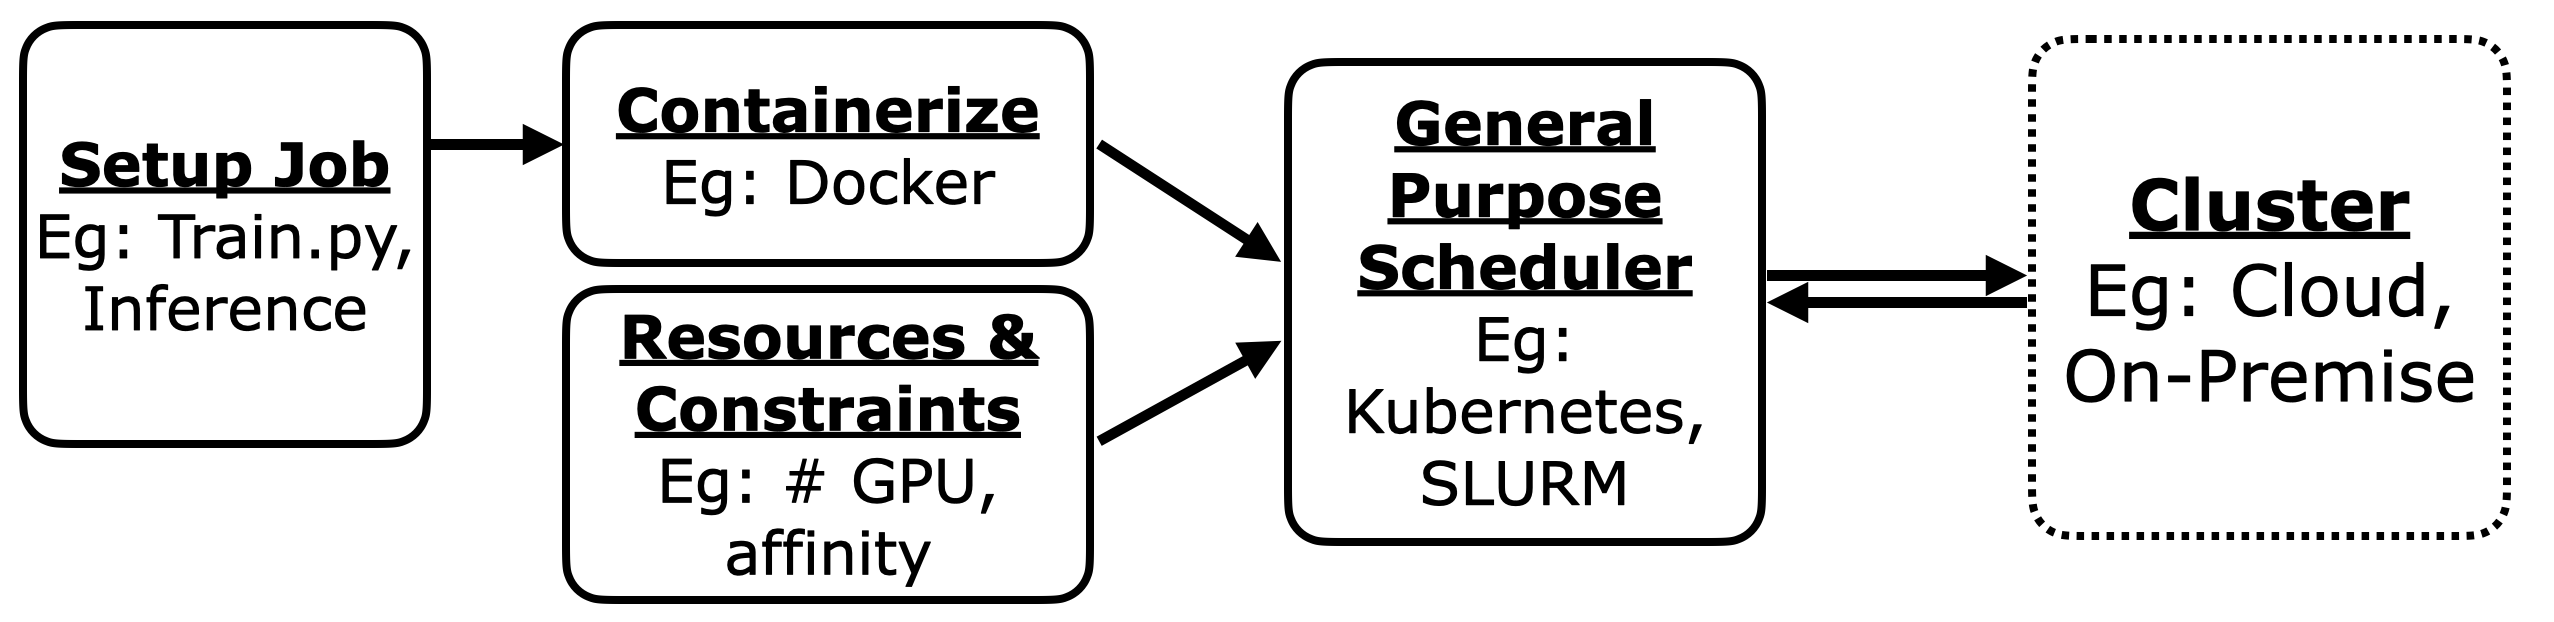
\includegraphics[height=2cm]{figures/workflow.png}}
\caption{A Typical Workflow }
\label{fig}
\end{figure}



\begin{enumerate}

\item Schedulers do not yet support fine-grained abstraction over GPUs like they
do with CPUs. Thus a job requiring GPU resources can acquire them only in
integer units, resulting in wastage \cite{kub1}.

\item Secondly, the responsibility of estimating the resource requirements
(memory/compute) is on the developer. Not surprisingly, demanding more resource
than strictly necessary is common practice. In addition, it takes significant
effort to design models and training mechanisms so as to make most of the
allotted GPU. This is tangential to expertise and objectives of the data
scientists \cite{nimble}

\end{enumerate}

\begin{figure*}
  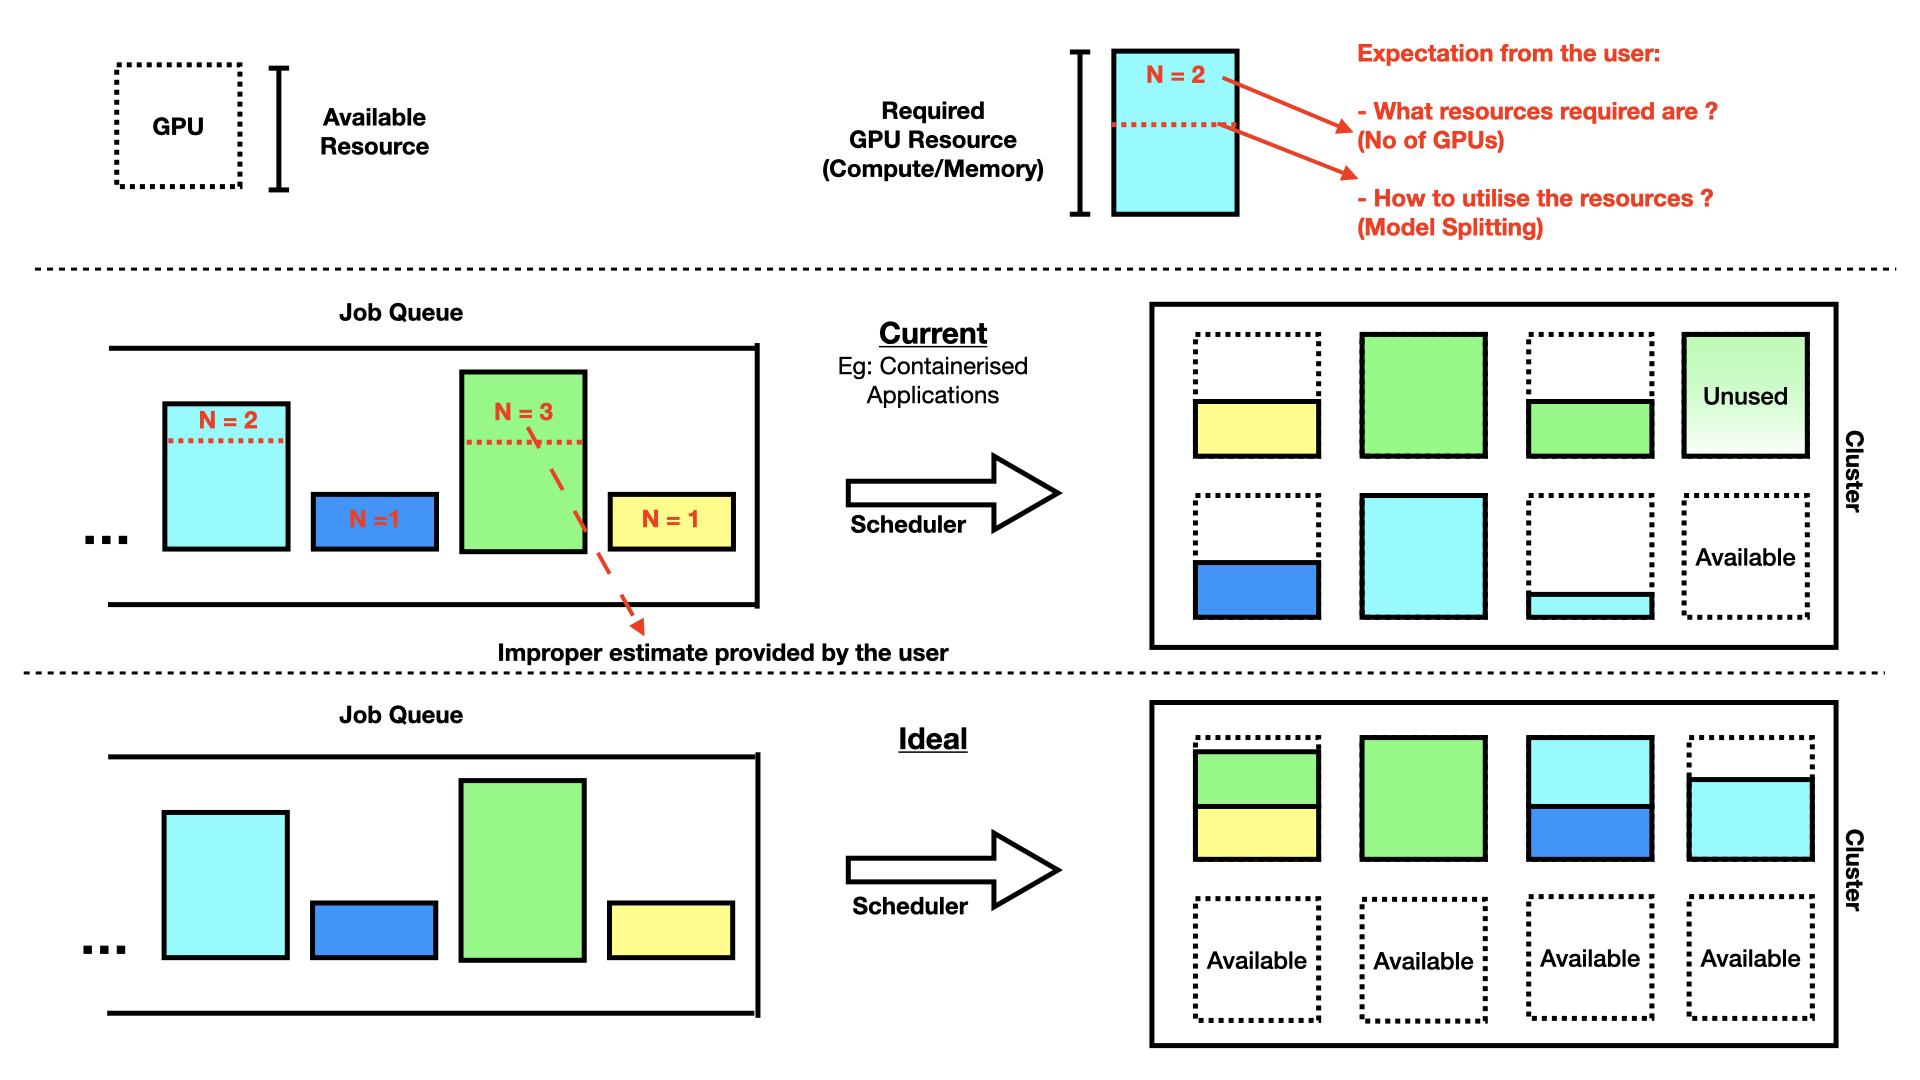
\includegraphics[width=\textwidth,height=8cm]{figures/pic.jpeg}
  \caption{Low cluster utilization by coarse-grained resource allocation and incorrect estimates. An Ideal system would require no such estimation and optimally pack jobs to exploit inherent parallelism in GPUs}
\end{figure*} 

The resulting inefficiencies is illustrated in Figure 1. This over-provisioning
coupled with low utilization of the provisioned resource leads to, as
\cite{delimitrou} puts it, ``mostly-allocated, but lightly-utilized systems".
This obviously has serious financial as well as developer productivity
implications, especially when most data science teams are small (>60\% have less
than 10 members \cite{kaggle})

This by no means is a new problem. A large body of recent works have suggested
improvements to cluster management tools by exploiting the special
characteristics of DL jobs. For instance AntMan \cite{antman} exploits the
periodic nature of resource consumption in model training to improve cluster
utilisation. Clockwork \cite{clockwork} exploits the predictable time duration
of DL tasks to design a scheduler. It is also worth noting that many of the
works are proprietary systems that address the problems in large companies like
Microsoft and Alibaba. The systems either build custom tools or accept the
integer-level granularity and instead focus on other aspects like fairness of
allocation or generality of the the jobs supported (eg: both Pytorch and
Tensorflow jobs ).  Even then, in systems like Gandiva \cite{gandiva} `job
packing' on a single GPU is one of the possible actions taken by the job
scheduler.


Recently there have been attempts to do allocation at sub-GPU level i.e sharing
jobs on the same GPU. For instance, startup run.ai \cite{runai} released a
feature to use fractional GPU resources directly through Kubernetes. A highlight
of Nvidia's Volta architecture and Multiprocess-Services \cite{mps} is the
ability for multiple processes to seamlessly share GPU memory and compute
resources. Memory leakage protection is also builtin. While these improvements
provide the substrate to utilize GPUs better, the systems still depend heavily
on the developers expertise. Nevertheless, fast evolving efforts in
virtualization of GPU only further validates the need for fine-grained
allocation of GPU resources. We ask, even if GPU virtualization is accessible to
a team, how can they make most of their hardware and do so transparently,
without requiring intervention of the developer. Thus, GPU virtualization will
make our work more reliable by making it easy to manage process boundaries.

We argue that Model Parallelism - the practice of dividing a model across
multiple GPU's - naturally arises in designing an efficient cluster management
system that granularly allots GPU resources. Further, drawing from our
learnings designing Baechi \cite{baechi} - a model splitting mechanism - we
build a scheduler that with properties of an ideal scheduler show in Figure 2.

Model Parallelism so far has been exclusively seen as a method to be used when
training a model that does not to fit in one single GPU or when using large
batch sizes (often data parallelism is preferred for the later case ).

Specifically, we highlight the following:

\begin{itemize}

\item Consider an incoming job to be scheduled on a cluster already running some
jobs. With the ability to do fine-grained allocation of GPU resources, the
problem of scheduling  is equivalent to model parallelism of the model over the
residual resources in the cluster

\item Model parallelism splits the computation graph of a DL job across multiple
GPUs with the objective of minimizing the training or inference step time.
However the same algorithms can be used to split computations within a GPU to
exploit the inherent parallelism of GPU, thus improving utilization. This
however requires careful design using streams \cite{nimble}

\item A resource estimation routine is an essential component of a model
splitting system like Baechi. This in turn frees the developer from the burden
of estimating the resource requirements.

\end{itemize}

Figure 2 shows the high level description of a scheduler inspired by this
approach. The grey highlight shows the blocks that constitutes current design of
Baechi. \cite{baechi}. In the report, we will look at how these different
components contribute towards building an ideal cluster management system as
described in Figure 1.

\begin{figure}[htbp]
\centerline{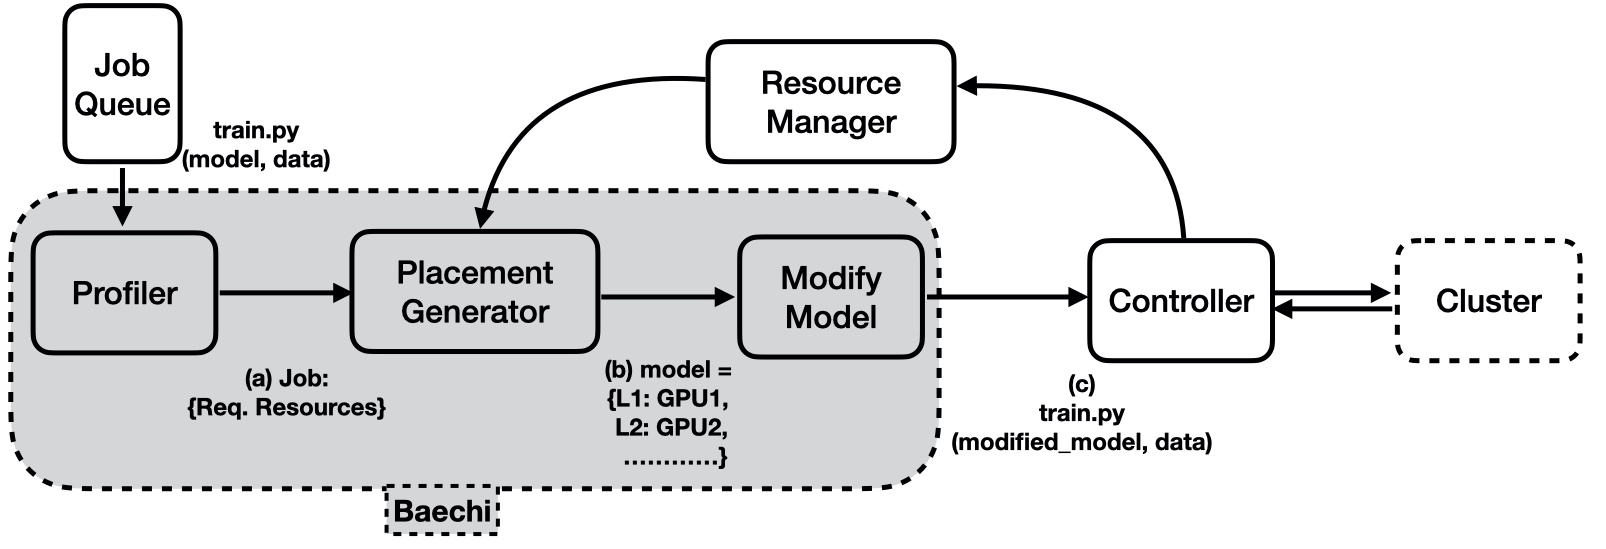
\includegraphics[height=3cm]{figures/baechi.jpg}}
\caption{High Level Design}
\label{fig3}
\end{figure}


